\chapter{Resultados}
%\markboth{\thechapter ~~~ Resultados}{}
%\label{result}

Neste capítulo, os resultados para o projeto descritos no capítulo anterior serão apresentados. A obtenção do modelo da 
planta foi dada de duas formas diferentes: por meio da convenção de \textit{Denavit-Hartenberg} e equações de 
\textit{Euler-Lagrange} e por meio do ensaio em malha aberta. Para o primeiro método, foram feitas algumas considerações,
estas seguem abaixo:
\begin{enumerate}
 \item O elo do cotovelo e o elo do ombro são barras de comprimento $L$ e massa $m$, e possuem o eixo de rotação no fim
 da barra;
 \item O elo da base é um cilindro sólido de raio $r$, altura $h$ e massa $m$;
 \item A distribuição de massa de cada elo com a sua junta respectiva é simétrica em relação à estrutura do corpo, ou seja,
 a massa está uniformemente distribuída ao longo do corpo.
\end{enumerate}

O código em MATLAB referente ao modelo obtido por meio da convenção de \textit{Denavit-Hartenberg} e equações de
\textit{Euler-Lagrange} é apresentado no \refanexo{anexo:denHatEulerLagr}. A \autoref{fig:dh_simulation} mostra 
o modelo encontrado por meio da matriz de homogeneidade resultante da convenção DH. Nota-se a coerência deste 
modelo com o manipulador real por respeitar a proporção e distribuição dos elos e juntas.

\begin{figure}[ht]
  \centering
  \caption{Gráfico da representação \textit{Denavit-Hartenberg} obtida}
  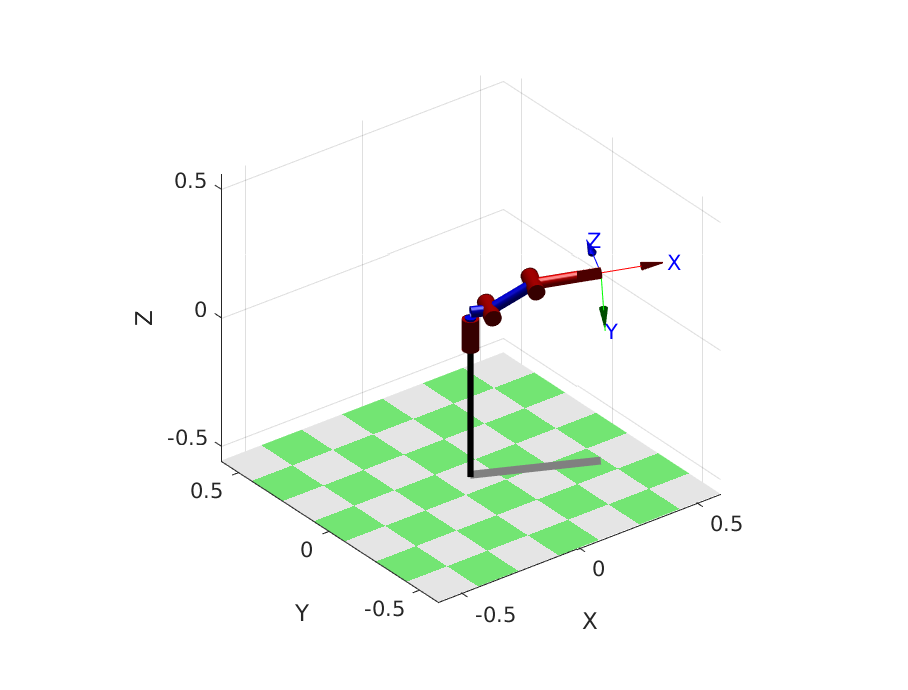
\includegraphics[width = 0.7\columnwidth]{Imagens/dh_simulation}
  \fonte{Do autor}
  \label{fig:dh_simulation} 
\end{figure}

As considerações citadas no início deste capítulo, em conjunto com a complexidade na obtenção dos Símbolos de \textit{Christoffel}
tornaram a modelagem EL inviável. A solução mais coerente encontrada foi a execução do ensaio em malha aberta para a obtenção do modelo 
de cada junta do manipulador, seguido do controle de junta independente

Os modelos da planta usados para projetar os controladores foram obtidos através de ensaios em malha aberta (MA) e seguem 
na próxima seção. Três modelos foram levantados: um para a base, um para o ombro e outro para o cotovelo, e para 
cada um deles foi projetado um controlador. Esse processo é conhecido na literatura como controle de juntas independentes.

\section{Ensaio em malha aberta}
\markright{\thesection ~~~ Resultado ensaio em malha aberta}

A comunicação com os servomotores foi feita inicialmente com um computador através da porta serial com o protocolo 
UART. A linguagem usada para a execução do ensaio em malha aberta foi o \textit{Python}, e seu código completo
encontra-se disponível em \cite{lelis_model}.

Para cada uma das juntas foi feita uma montagem semelhante a apresentada na \autoref{fig:diagEnsaioMA}. Foi aplicada na entrada de
cada um dos servomotores uma referência em degrau para o ângulo $\theta$ (em graus). Inicialmente, o sistema tinha sido
configurado para um tempo de amostragem de $0,01s$. De acordo com a resposta obtida, observou-se uma superamostragem dos dados,
e, devido a isso, o tempo de amostragem foi reajustado empiricamente para $0,23s$. Os ângulos de resposta (em graus) obtidos
ao longo do tempo para cada uma das juntas são apresentados na \autoref{fig:ensaioMalhaAberta}.

\begin{figure}[h!]
  
  \centering
  \caption{Gráficos da entrada e resposta para o ensaio em MA de cada uma das juntas}
  \begin{subfigure}{.5\textwidth}
    \centering
    \caption{Base}
    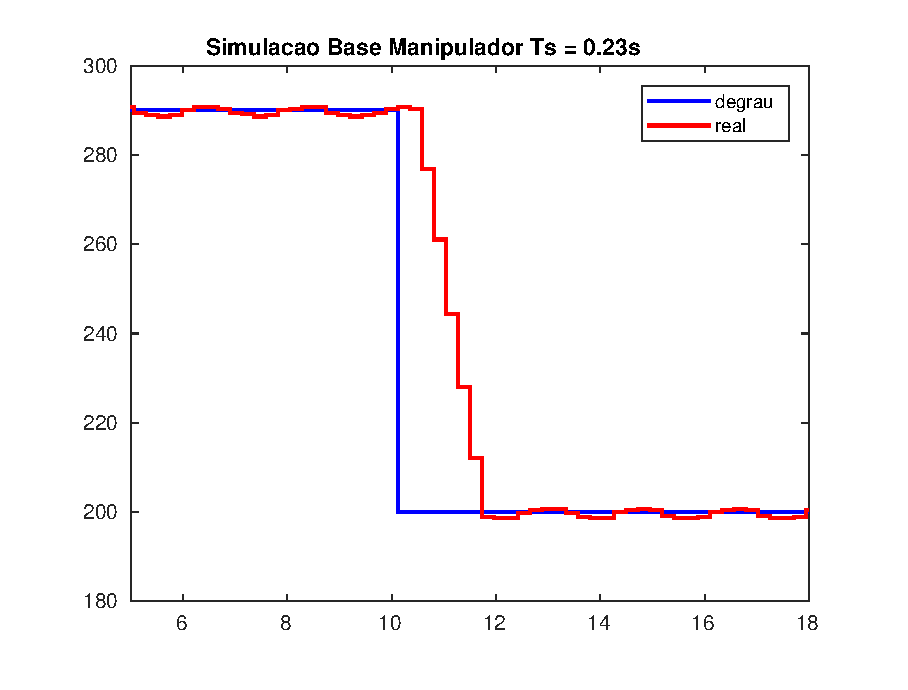
\includegraphics[width = 1\columnwidth]{Imagens/base_ma}
    \fonte{Do autor}
    \label{fig:base_ma}
  \end{subfigure}%
  \begin{subfigure}{.5\textwidth}
    \centering
    \caption{Ombro}
    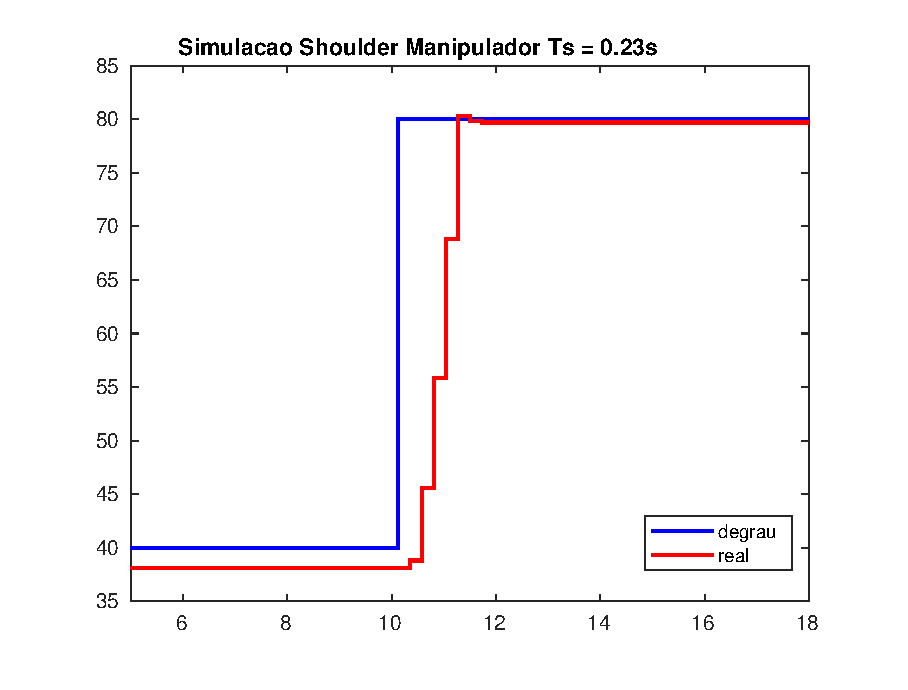
\includegraphics[width = 1\columnwidth]{Imagens/shoulder_ma}
    \fonte{Do autor}
    \label{fig:shoulder_ma}
  \end{subfigure}%
  
  \label{fig:ensaioMalhaAberta} 
  
\end{figure}

\begin{figure}[h!]\ContinuedFloat
  \begin{subfigure}{\textwidth}
    \centering
    \caption{Cotovelo}
    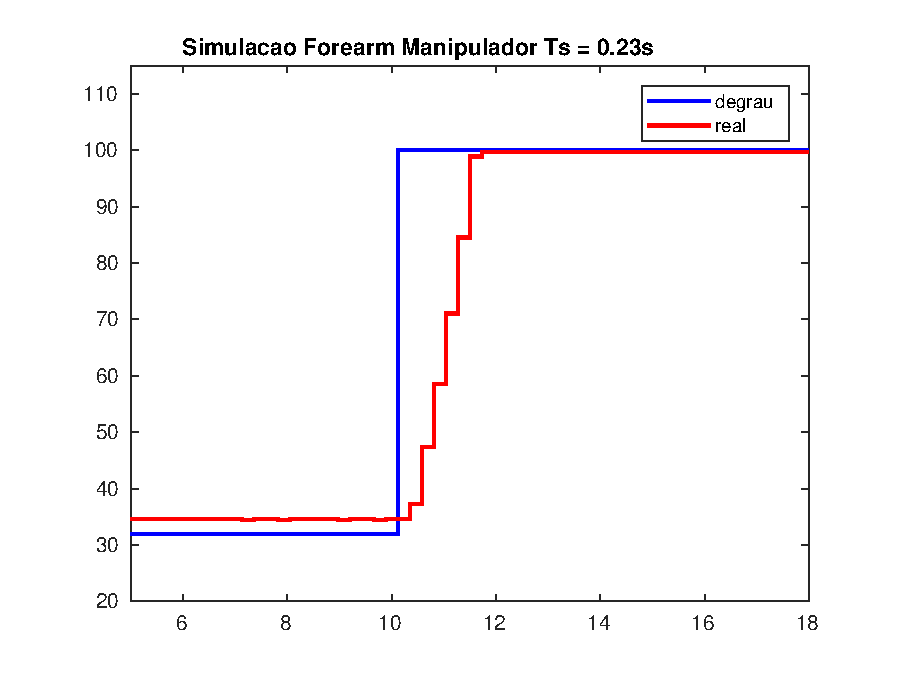
\includegraphics[width = 0.55\columnwidth]{Imagens/forearm_ma}
    \fonte{Do autor}
    \label{fig:forearm_ma}
  \end{subfigure}%
\end{figure}

A princípio, observando as respostas em malha aberta das juntas, a dinâmica de cada uma poderia ser aproximada por
um modelo de primeira ordem. Entretanto, constatou-se experimentalmente que um modelo de segunda ordem, 
conforme \eqref{eq:sistemaSegundaOrdem}, era mais apropriado para descrever a dinâmica de cada junta do sistema.
Tal fato se deve, possivelmente, ao controlador interno presente nos servomotores.

Observando as Figuras \ref{fig:base_ma} e \ref{fig:forearm_ma}, observa-se um comportamento próximo do 
amortecimento crítico. Quando ocorre esse tipo de comportamento, pode-se escolher $\xi=1$ na função de 
transferência. Por outro lado, em \ref{fig:shoulder_ma}, observa-se
um pequeno sobressinal, o que resulta em um $\xi$ menor, aproximando-se para este caso: $\xi = 0,8$.

O tempo de acomodação, definido em \eqref{eq:tempoAcomodacao}, variou para todas as juntas na 
faixa $0,9s < t_s < 1,3s$. De acordo com testes qualitativos para a validação do modelo, e pelas Figuras 
\ref{fig:base_ma}, \ref{fig:shoulder_ma} e \ref{fig:forearm_ma}, foi considerado para a base, ombro e
cotovelo respectivamente: $t_s = 1,0952s$, $t_s = 0,9333s$, $t_s = 1,0952s$. Dessa forma, substituindo em 
\eqref{eq:tempoAcomodacao} as constantes encontradas por aproximação, obtém-se para as frequências naturais de
oscilação ($\omega_n$) da base, ombro e
cotovelo respectivamente: $\omega_n = 3.6522 rad/s$, $\omega_n = 5.3571 rad/s$, $\omega_n = 3.6522 rad/s$.
O valor das variáveis encontradas para cada uma das juntas segue na \autoref{tab:ctesModeloMA}

\begin{center}
    \captionof{table}{Constantes determinadas para os modelos das juntas}
    \begin{tabular}{| c | c | c | c |}\hline
      \textbf{Junta}	& $\xi$ 	& $t_s$ (s)	& $\omega_n$ (rad/s)	\\ \hline
      Base		& 1 		& 1,0952	& 3,6522		\\ \hline
      Ombro		& 0,8 		& 0,9333	& 5,3571		\\ \hline
      Cotovelo		& 1 		& 1,0952	& 3,6522		\\ \hline
    \end{tabular}
    \label{tab:ctesModeloMA}
\end{center}

\section{Fase 1 da técnica HIL}
\markright{\thesection ~~~ Fase 1 da técnica HIL}

Como foi exposto na seção anterior, as constantes foram encontradas por aproximações de acordo
com o que foi observado no ensaio em malha aberta. A partir disso, as funções de transferência
para a base, ombro e cotovelo foram obtidas através da Equação \eqref{eq:sistemaSegundaOrdem} e 
seguem respectivamente em \eqref{eq:baseModel}, \eqref{eq:shoulderModel} e \eqref{eq:forearmModel}:
\begin{equation}
  \begin{gathered}
    G(s) = \frac{13,3384}{s^2 + 7,3043s + 13,3384}
  \end{gathered}
  \label{eq:baseModel}
\end{equation}

\begin{equation}
  \begin{gathered}
    G(s) = \frac{0,9965 \cdot 28,69898}{s^2 + 8,5714s + 28,69898}
  \end{gathered}
  \label{eq:shoulderModel}
\end{equation}

\begin{equation}
  \begin{gathered}
   G(s) = \frac{13,3384}{s^2 + 7,3043s + 13,3384}
  \end{gathered}
  \label{eq:forearmModel}
\end{equation}

Os mesmos degraus aplicados na planta real, foram aplicados nas funções de transferência para
validação dos modelos. Os resultados obtidos seguem na \autoref{fig:base_ma_simul}, na
\autoref{fig:shoulder_ma_simul} e na \autoref{fig:forearm_ma_simul}.

\begin{figure}[h!]
  
  \centering
  \caption{Gráficos da entrada e resposta do modelo obtido para cada uma das juntas}
  \begin{subfigure}{.5\textwidth}
    \centering
    \caption{Base}
    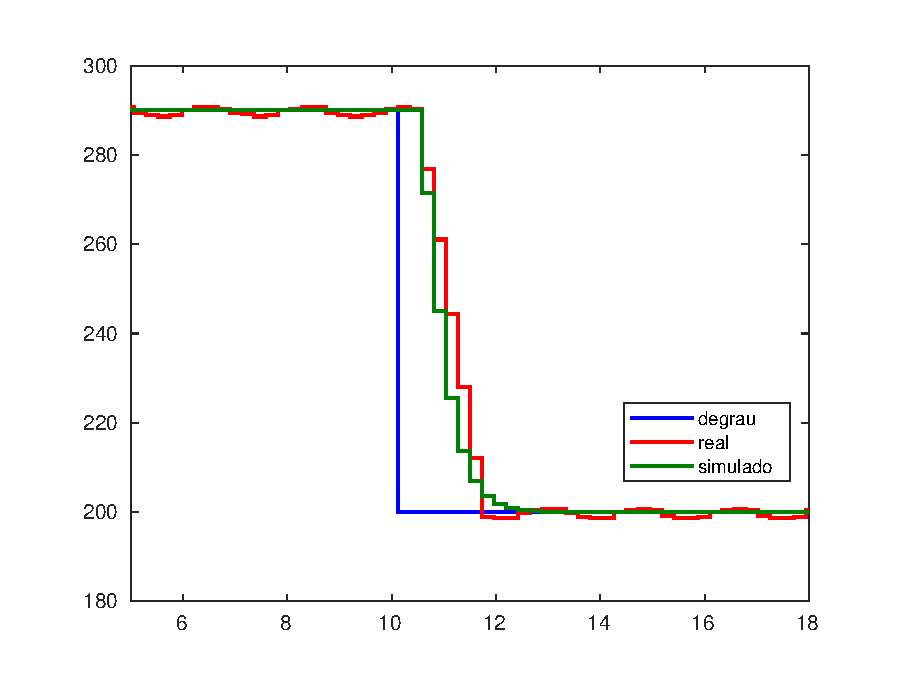
\includegraphics[width = .8\columnwidth]{Imagens/base_ma_simul}
    \fonte{Do autor}
    \label{fig:base_ma_simul}
  \end{subfigure}%
  \begin{subfigure}{.5\textwidth}
    \centering
    \caption{Ombro}
    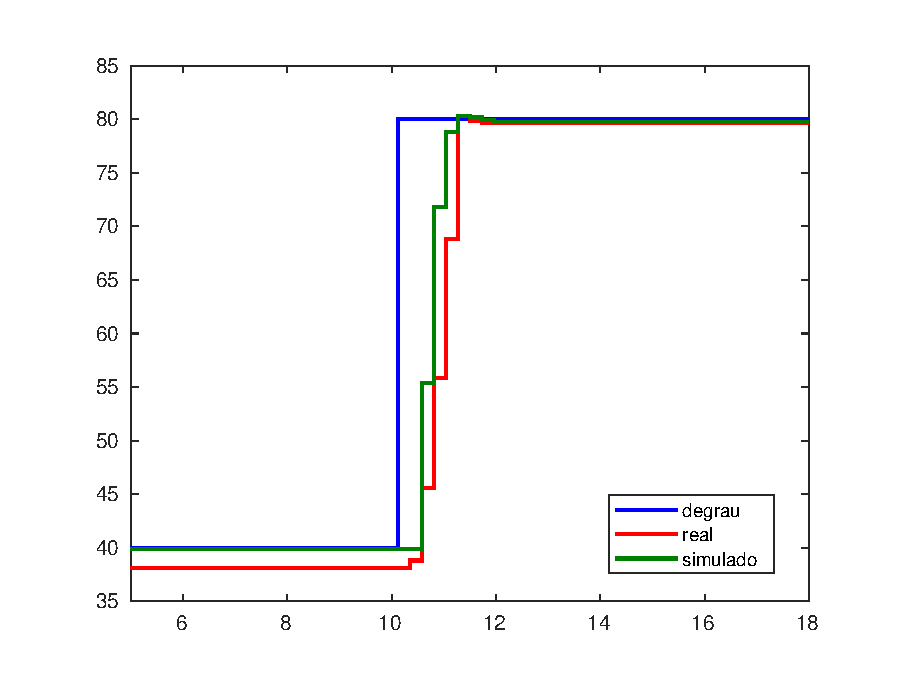
\includegraphics[width = .8\columnwidth]{Imagens/shoulder_ma_simul}
    \fonte{Do autor}
    \label{fig:shoulder_ma_simul}
  \end{subfigure}%
  \\
  \begin{subfigure}{\textwidth}
    \centering
    \caption{Cotovelo}
    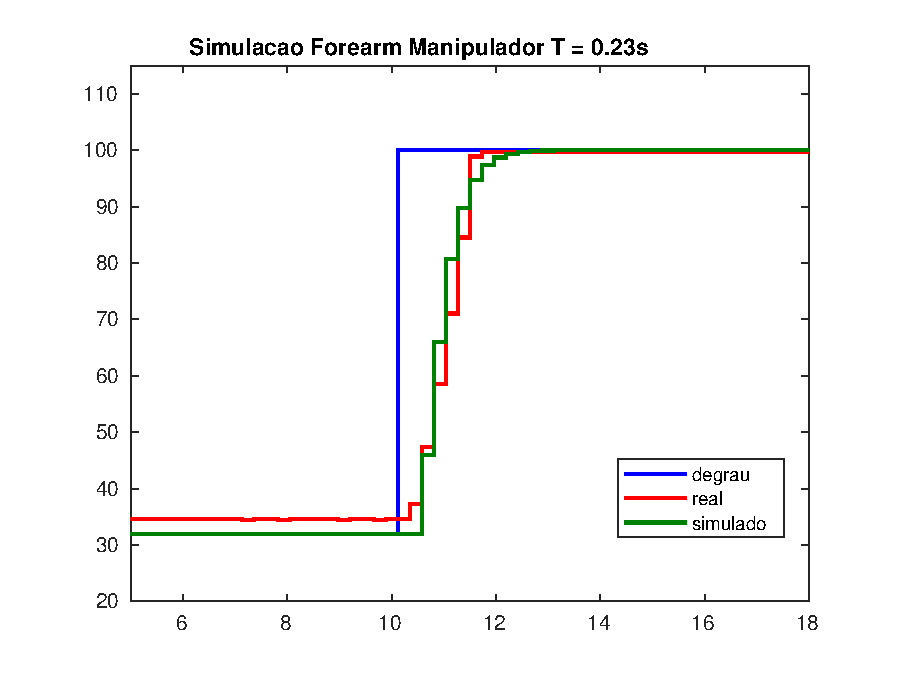
\includegraphics[width = 0.4\columnwidth]{Imagens/forearm_ma_simul}
    \fonte{Do autor}
    \label{fig:forearm_ma_simul}
  \end{subfigure}%
  
  \label{fig:ensaioMalhaAbertaSimul} 

\end{figure}

Note que as curvas simuladas aproximam adequadamente as respostas de cada junta em malha aberta. Assim, 
conclui-se que os modelos obtidos são satisfatórios para representar as dinâmicas das juntas do manipulador.

Obtidos os modelos que descrevem as dinâmicas das juntas, a próxima etapa da fase 1 da técnica HIL foi o projeto dos 
controladores pelo método do lugar das raízes. Considerando que as especificações do projeto
de controle seriam atendidas caso houvesse um baixo sobressinal na resposta, e o erro em estado
estacionário igual a
zero. Dadas as características do modelo da planta, verificou-se experimentalmente que um controlador
PI seria suficiente para atender as especificações de projeto. Esse controlador é obtido a partir
de \eqref{eq:pid} escolhendo $T_d=0$.
Assim sendo, na análise do lugar das raízes (através da ferramenta \textit{sisotool} do \textit{Matlab}), foi colocado um polo de malha
fechada na origem e um zero no eixo real para o controlador de cada uma das juntas. O ganho foi 
ajustado de tal forma que os polos de malha fechada ficassem o mais próximo possível do eixo real (parte complexa próxima de zero), 
assim a resposta apresentaria pouca ou nenhuma oscilação ao fechar a malha. A partir dessas considerações de projeto, 
obtiveram-se os controladores para a base, ombro e cotovelo dados respectivamente por \eqref{eq:base_ctrl}, \eqref{eq:shoulder_ctrl}
e \eqref{eq:forearm_ctrl}:
\begin{equation}
  \begin{gathered}
    C(s) = \frac{0,152s + 0,8}{s}
  \end{gathered}
  \label{eq:base_ctrl}
\end{equation}
\begin{equation}
  \begin{gathered}
    C(s) = \frac{0,413 s + 0,9229}{s}
  \end{gathered}
  \label{eq:shoulder_ctrl}
\end{equation}
\begin{equation}
  \begin{gathered}
   C(s) = \frac{0,152s + 0,8}{s}
  \end{gathered}
  \label{eq:forearm_ctrl}
\end{equation}

O código de simulação completo com as funções de transferência e os controladores projetados encontra-se em \cite{lelis_hil1}.
Ao fechar as malhas, os resultados obtidos para o modelo da planta e para a planta física seguem na 
\autoref{fig:base_mf_simul}, na \autoref{fig:shoulder_mf_simul} e na \autoref{fig:forearm_mf_simul}.

\begin{figure}[h!]
  
  \centering
  \caption{Gráficos das respostas ao degrau em malha fechada - HIL Fase 1}
  \begin{subfigure}{.5\textwidth}
    \centering
    \caption{Base}
    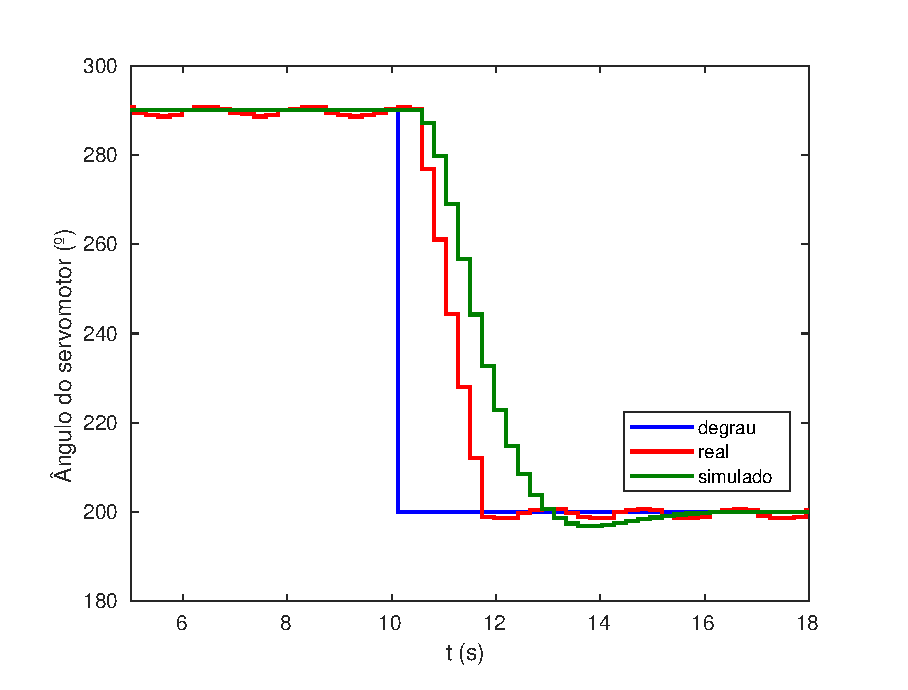
\includegraphics[width = .78\columnwidth]{Imagens/base_mf_simul}
    \fonte{Do autor}
    \label{fig:base_mf_simul}
  \end{subfigure}%
  \begin{subfigure}{.5\textwidth}
    \centering
    \caption{Ombro}
    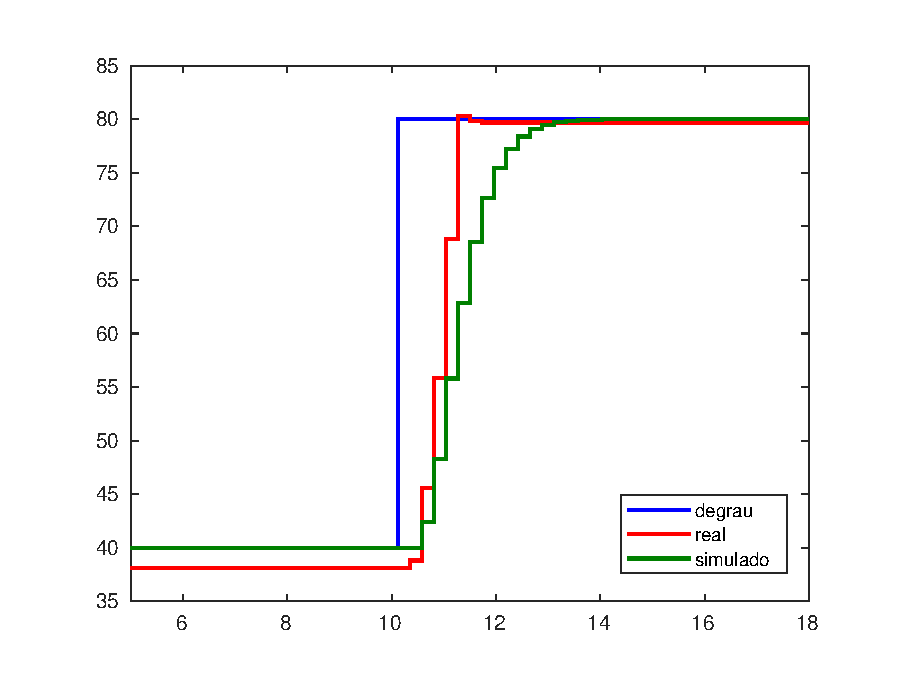
\includegraphics[width = .75\columnwidth]{Imagens/shoulder_mf_simul}
    \fonte{Do autor}
    \label{fig:shoulder_mf_simul}
  \end{subfigure}%
  
  \label{fig:malhaFechadaHil1} 
  
\end{figure}

\begin{figure}[h!]\ContinuedFloat
  \begin{subfigure}{\textwidth}
    \centering
    \caption{Cotovelo}
    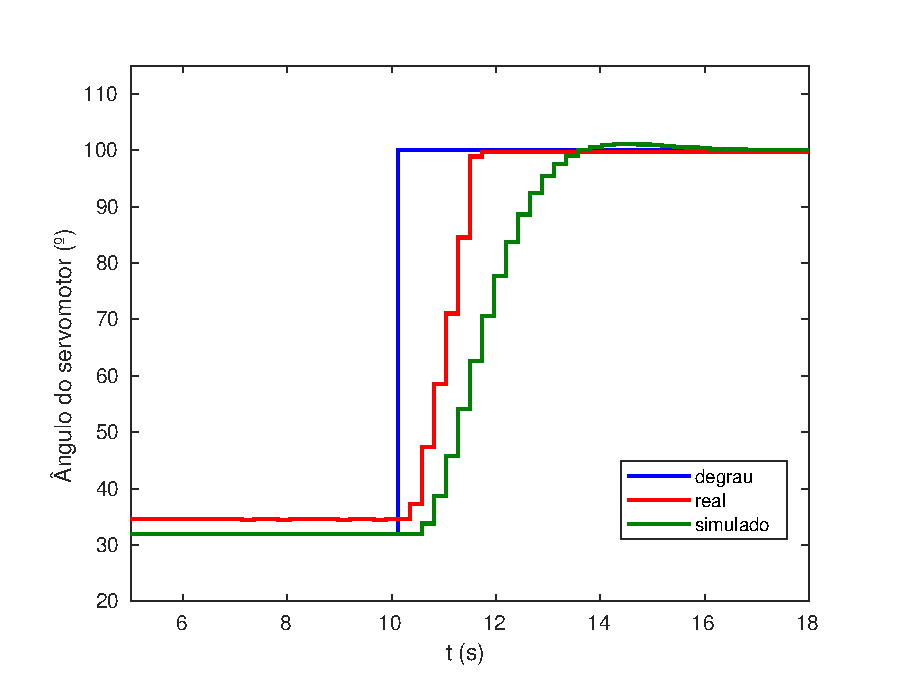
\includegraphics[width = 0.55\columnwidth]{Imagens/forearm_mf_simul}
    \fonte{Do autor}
    \label{fig:forearm_mf_simul}
  \end{subfigure}%

\end{figure}

%Com o primeiro controlador projetado para a base e para o cotovelo, ao fechar a malha, a resposta não apresentava
%sobresinal como mostrado na \autoref{fig:base_mf_simul} e na \autoref{fig:forearm_mf_simul}. Apesar disso,
%ao passar para o domínio discreto, o controlador passava a ter um zero não mínimo. E como foi citado 
%anteriormente, o zero não mínimo é um comportamento indesejado para o sistema, por esse motivo, o controlador
%de ambas as juntas foi alterado.

Nota-se na \autoref{fig:malhaFechadaHil1} que as respostas obtidas em malha fechada possuem uma dinâmica mais lenta,
isso se deve à não necessidade de uma resposta rápida, mas sim, à necessidade de uma transição mais suave. Outro fator
levado em consideração ao fechar a malha foi a obtenção do erro em estado estacionário igual a zero. Em malha aberta, a base 
apresentava uma variação em torno do estado estacionário infindável, ao fechar a malha essa variação foi corrigida quando o
sistema entra em estado estacionário.

\section{Fase 2 da técnica HIL}
\markright{\thesection ~~~ Fase 2 da técnica HIL}

Como o sinal da resposta da planta é amostrado periodicamente pela placa de aquisição de dados do
computador e pela \textit{Raspberry Pi}, torna-se necessária a discretização do controlador e da planta simulada. A 
discretização foi feita através do comando \textit{c2d( )} do \textit{Matlab} utilizando um segurador de 
ordem zero e com um tempo de amostragem de $0,23s$. O resultado da discretização para as juntas e os respectivos
controladores segue a seguir.
Para a base:
\begin{equation}
  \begin{gathered}
    G(z) = \frac{0,8273z - 0,6543}{z^2 - 0,9515z + 0,1245} \quad \text{e} \quad C(z) = \frac{0,152z + 0,032}{z - 1}
  \end{gathered}
  \label{eq:base_discrete}
\end{equation}
para o ombro:
\begin{equation}
  \begin{gathered}
    G(z) = \frac{0,3876z - 0,198}{z^2 - 0,5515z + 0,1393} \quad \text{e} \quad C(z) = \frac{0,1572z + 0,06513}{z - 1}
  \end{gathered}
  \label{eq:shoulder_discrete}
\end{equation}
para o cotovelo:
\begin{equation}
  \begin{gathered}
   G(z) = \frac{0,8273z - 0,6543}{z^2 - 0,9515z + 0,1245} \quad \text{e} \quad C(z) = \frac{0,152z + 0,032}{z - 1}
  \end{gathered}
  \label{eq:forearm_discrete}
\end{equation}

O próximo passo foi a obtenção da equação a diferenças para cada uma das plantas e
controladores. Para isso, foi feito o seguinte procedimento para o modelo da base e seu respectivo controlador:

\begin{equation*}
  \begin{gathered}
    G(z) = \frac{0,8273z - 0,6543}{z^2 - 0,9515z + 0,1245} \\[0.5cm]
    \frac{Y(z)}{U(z)} = \frac{0,8273z - 0,6543}{z^2 - 0,9515z + 0,1245}\\[0.5cm]
    \frac{Y(z)}{U(z)} = \frac{0,8273/z - 0,6543/z^2}{1 - 0,9515/z + 0,1245/z^2}\\[0.5cm]
    Y(z) - \frac{0,9515}{z} \;Y(z) + \frac{0,1245}{z^2} \;Y(z) = \frac{0,8273}{z} \;U(z) - \frac{0,6543}{z^2} \;U(z)
  \end{gathered}
  \label{eq:base_plant_diffEqIntro}
\end{equation*}
\begin{equation}
  \begin{gathered}
    y(k) = 0,8273 \;u(k-1) - 0,6543 \;u(k-2) + 0,9515 \;y(k-1) - 0,1245 \;y(k-2)
  \end{gathered}
  \label{eq:base_plant_diffEq}
\end{equation}

\begin{equation*}
  \begin{gathered}
    C(z) = \frac{0,152z + 0,032}{z - 1}\\[0.5cm]
    \frac{U(z)}{E(z)} = \frac{0,152z + 0,032}{z - 1}\\[0.5cm]
    \frac{U(z)}{E(z)} = \frac{0,152 + 0,032/z}{1 - 1/z}\\[0.5cm]
    U(z) - \frac{U(z)}{z} = 0,152\;E(z) + \frac{0,032}{z}\;E(z)\\[0.5cm]
  \end{gathered}
  \label{eq:base_ctrl_diffEqIntro}
\end{equation*}
\begin{equation}
  \begin{gathered}
    u(k) = u(k-1) + 0,152\; e(k) + 0,032 \;e(k-1)
  \end{gathered}
  \label{eq:base_ctrl_diffEq}
\end{equation}

O procedimento elucidado acima é repetido para os modelos e controladores do ombro \eqref{eq:shouder_plant_diffEq} - \eqref{eq:shouder_ctrl_diffEq} 
e do cotovelo \eqref{eq:forearm_plant_diffEq} - \eqref{eq:forearm_ctrl_diffEq}, resultando nos seguintes pares de equações a diferenças:
\begin{equation}
  \begin{gathered}
    y(k) = 0,3876 u(k-1) + 0,198 u(k-2) + 0,5515 y(k-1) - 0,1393 y(k-2)
  \end{gathered}
  \label{eq:shouder_plant_diffEq}
\end{equation}
\begin{equation}
  \begin{gathered}
    u(k) = u(k-1) + 0,1572  e(k) + 0,06513 e(k-1)
  \end{gathered}
  \label{eq:shouder_ctrl_diffEq}
\end{equation}
\begin{equation}
  \begin{gathered}
    y(k) = 0,8273 u(k-1) - 0,6543 u(k-2) + 0,9515y(k-1) - 0,1245y(k-2)
  \end{gathered}
  \label{eq:forearm_plant_diffEq}
\end{equation}
\begin{equation}
  \begin{gathered}
    u(k) = u(k-1) + 0,152 e(k) + 0,032 e(k-1)
  \end{gathered}
  \label{eq:forearm_ctrl_diffEq}
\end{equation}

% para a planta do ombro:
% 
% \begin{equation*}
%   \begin{gathered}
%     G(z) = \frac{0,3876 z + 0,198}{z^2 - 0,5515 z + 0,1393} \\[0.5cm]
%     \frac{Y(z)}{U(z)} = \frac{0,3876 z + 0,198}{z^2 - 0,5515 z + 0,1393}\\[0.5cm]
%     \frac{Y(z)}{U(z)} = \frac{0,3876/z + 0,198/z^2}{1 - 0,5515/z + 0,1393/z^2}\\[0.5cm]
%     Y(z) - \frac{0,5515}{z} \;Y(z) + \frac{0,1393}{z^2} \;Y(z) = \frac{0,3876}{z} \;U(z) + \frac{0,198}{z^2} \;U(z)
%   \end{gathered}
%   \label{eq:shouder_plant_diffEqIntro}
% \end{equation*}
% \begin{equation}
%   \begin{gathered}
%     y(k) = 0,3876 \;u(k-1) + 0,198 \;u(k-2) + 0,5515 \;y(k-1) - 0,1393 \;y(k-2)
%   \end{gathered}
%   \label{eq:shouder_plant_diffEq}
% \end{equation}
% para o controlador do ombro:
% 
% \begin{equation*}
%   \begin{gathered}
%     C(z) = \frac{0,1572 z + 0,06513}{z - 1}\\[0.5cm]
%     \frac{U(z)}{E(z)} = \frac{0,1572 z + 0,06513}{z - 1}\\[0.5cm]
%     \frac{U(z)}{E(z)} = \frac{0,1572 + 0,06513/z}{1 - 1/z}\\[0.5cm]
%     U(z) - \frac{U(z)}{z} = 0,1572 \;E(z) + \frac{0,06513}{z}\;E(z)\\[0.5cm]
%   \end{gathered}
%   \label{eq:shouder_ctrl_diffEqIntro}
% \end{equation*}
% \begin{equation}
%   \begin{gathered}
%     u(k) = u(k-1) + 0,1572 \; e(k) + 0,06513 \;e(k-1)
%   \end{gathered}
%   \label{eq:shouder_ctrl_diffEq}
% \end{equation}
% para a planta do cotovelo:
% 
% \begin{equation*}
%   \begin{gathered}
%     G(z) = \frac{0,8273z - 0,6543}{z^2 - 0,9515z + 0,1245} \\[0.5cm]
%     \frac{Y(z)}{U(z)} = \frac{0,8273z - 0,6543}{z^2 - 0,9515z + 0,1245}\\[0.5cm]
%     \frac{Y(z)}{U(z)} = \frac{0,8273/z - 0,6543/z^2}{1 - 0,9515/z + 0,1245/z^2}\\[0.5cm]
%     Y(z) - \frac{0,9515}{z} \;Y(z) + \frac{0,1245}{z^2} \;Y(z) = \frac{0,8273}{z} \;U(z) - \frac{0,6543}{z^2} \;U(z)
%   \end{gathered}
%   \label{eq:forearm_plant_diffEqIntro}
% \end{equation*}
% \begin{equation}
%   \begin{gathered}
%     y(k) = 0,8273 \;u(k-1) - 0,6543 \;u(k-2) + 0,9515 \;y(k-1) - 0,1245 \;y(k-2)
%   \end{gathered}
%   \label{eq:forearm_plant_diffEq}
% \end{equation}
% para o controlador do cotovelo:
% 
% \begin{equation*}
%   \begin{gathered}
%     C(z) = \frac{0,152z + 0,032}{z - 1}\\[0.5cm]
%     \frac{U(z)}{E(z)} = \frac{0,152z + 0,032}{z - 1}\\[0.5cm]
%     \frac{U(z)}{E(z)} = \frac{0,152 + 0,032/z}{1 - 1/z}\\[0.5cm]
%     U(z) - \frac{U(z)}{z} = 0,152\;E(z) + \frac{0,032}{z}\;E(z)\\[0.5cm]
%   \end{gathered}
%   \label{eq:forearm_ctrl_diffEqIntro}
% \end{equation*}
% \begin{equation}
%   \begin{gathered}
%     u(k) = u(k-1) + 0,152\; e(k) + 0,032 \;e(k-1)
%   \end{gathered}
%   \label{eq:forearm_ctrl_diffEq}
% \end{equation}

Determinadas as equações a diferenças, foi necessário realizar a montagem conforme a 
\autoref{fig:solucaoModelo}, isto é, configurar a conexão UART entre o computador e a 
\textit{Raspberry Pi}, e escrever o código em \textit{Python} para a planta simulada e
para o controlador que passou a rodar na \textit{Raspberry Pi} \cite{lelis_hil2}. Com isso,
a parte referente à simulação da planta ficou conforme o que segue: \\

\begin{lstlisting}[language=Python]
	# BASE - Funcao de transferencia da planta
	y_k[0] = 0.8273*u_k_delay[0] - 0.6543*u_k_delay_2[0]
	  + 0.9515*y_k_delay[0] - 0.1245*y_k_delay_2[0]

	# SHOULDER - Funcao de transferencia da planta
	y_k[1] = 0.3876*u_k_delay[1] + 0.198*u_k_delay_2[1]
	  + 0.5515*y_k_delay[1] - 0.1393*y_k_delay_2[1];

	# FOREARM - Funcao de transferencia da planta
	y_k[2] = 0.8273*u_k_delay[2] - 0.6543*u_k_delay_2[2]
	  + 0.9515*y_k_delay[2] - 0.1245*y_k_delay_2[2];
\end{lstlisting}
e do lado do controlador na \textit{Raspberry Pi}: \\

\begin{lstlisting}[language=Python]
	# BASE - Funcao de transferencia do controlador
	u_k[0] = u_k_delay[0] + 0.152*e_k[0] + 0.032*e_k_delay[0]

	# SHOULDER - Funcao de transferencia do controlador
	u_k[1] = u_k_delay[1] + 0.1572*e_k[1] + 0.06513*e_k_delay[1]

	# FOREARM - Funcao de transferencia do controlador
	u_k[2] = u_k_delay[2] + 0.152*e_k[2] + 0.032*e_k_delay[2]
\end{lstlisting}

Foram aplicadas as mesmas referências em degrau da primeira fase da técnica HIL para 
cada uma das plantas simuladas. Assim, as saídas obtidas ao longo do tempo para 
a fase 2 da técnica HIL são apresentadas nas Figuras \ref{fig:base_hilFase2}, 
\ref{fig:shoulder_hilFase2} e \ref{fig:forearm_hilFase2}.

\newpage

\begin{figure}[h!]
  
  \centering
  \caption{Gráficos das respostas ao degrau em malha fechada - HIL Fase 2}
  \begin{subfigure}{.5\textwidth}
    \centering
    \caption{Base}
    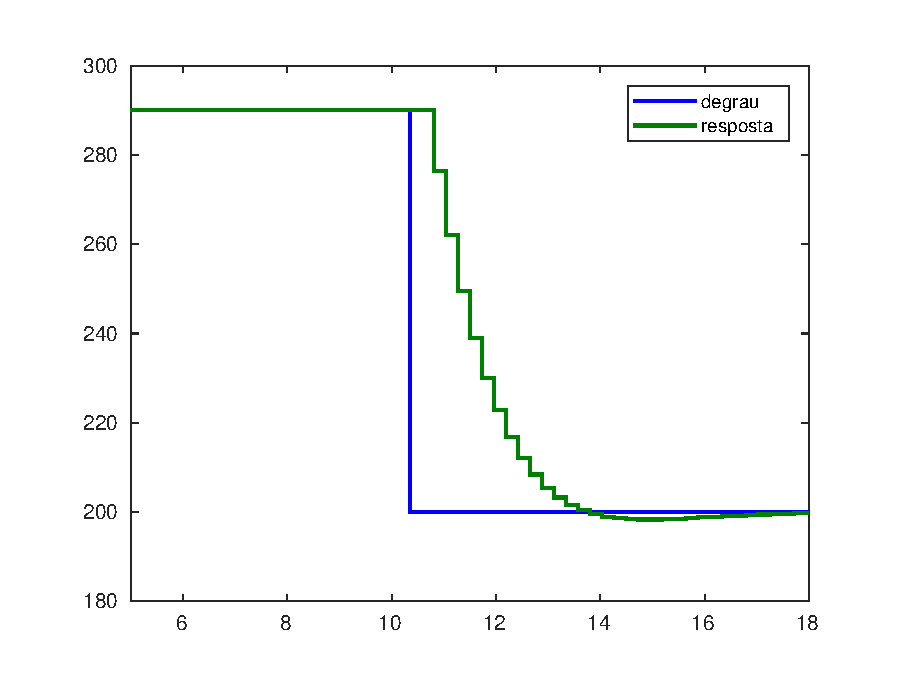
\includegraphics[width = 1\columnwidth]{Imagens/base_hilFase2}
    \fonte{Do autor}
    \label{fig:base_hilFase2}
  \end{subfigure}%
  \begin{subfigure}{.5\textwidth}
    \centering
    \caption{Ombro}
    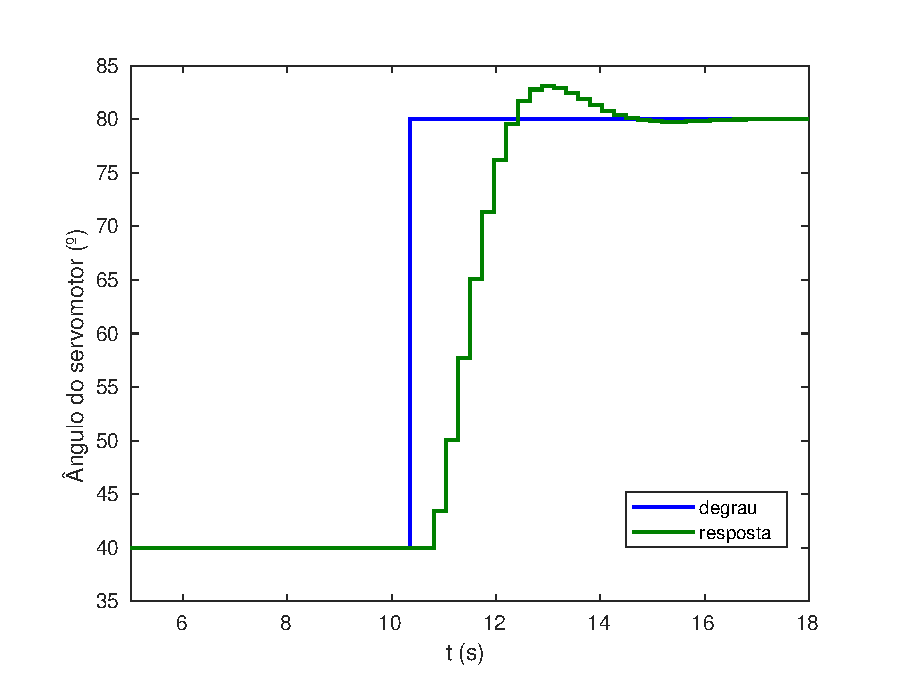
\includegraphics[width = 1\columnwidth]{Imagens/shoulder_hilFase2}
    \fonte{Do autor}
    \label{fig:shoulder_hilFase2}
  \end{subfigure}%
  \\[5ex]
  \begin{subfigure}{\textwidth}
    \centering
    \caption{Cotovelo}
    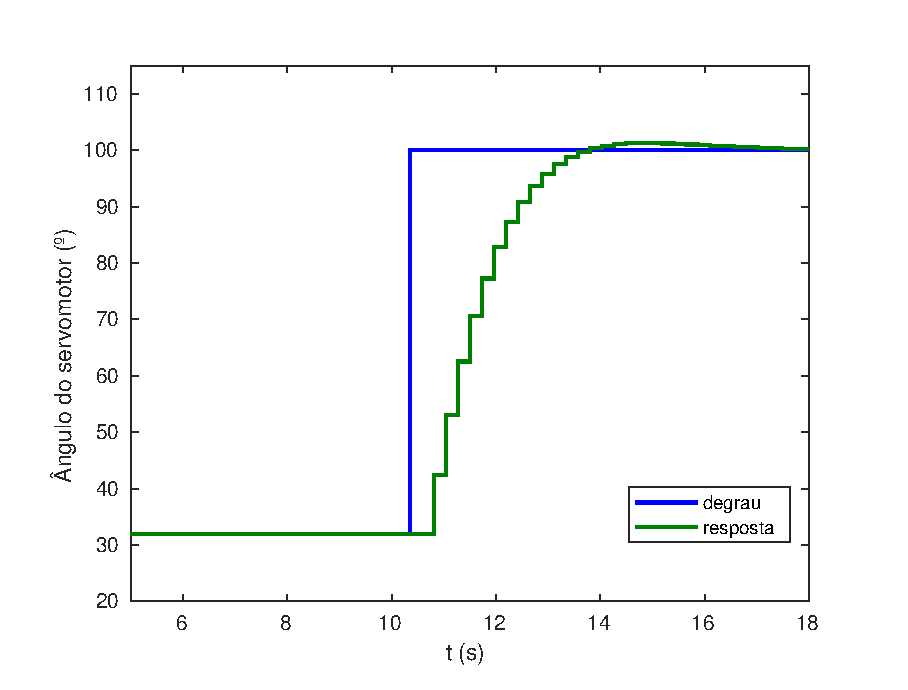
\includegraphics[width = 0.55\columnwidth]{Imagens/forearm_hilFase2}
    \fonte{Do autor}
    \label{fig:forearm_hilFase2}
  \end{subfigure}%
  
  \label{fig:hilFase2} 

\end{figure}

\section{Fase 3 da técnica HIL}
\markright{\thesection ~~~ Fase 3 da técnica HIL}

A última etapa da técnica HIL consiste em conectar o controlador implementado e validado 
na \textit{Raspberry Pi} e conectá-lo à malha de controle da planta do
manipulador, conforme a \autoref{fig:solucaoPlanta}. Além disso, foi necessário configurar
um ambiente de comunicação serial UART com os servomotores do manipulador. Para isso, uma
biblioteca em \textit{Python} foi utilizada. A parte do código referente à geração do sinal 
de controle é apresentada abaixo, sendo que o código completo encontra-se disponível 
em \cite{lelis_hil3}.\\[2cm]

\begin{lstlisting}[language=Python]
	def get_U_k(self, y_k):
		# Calcula lei de controle
		r_k = self.reference
		e_k = r_k - y_k
		
		# Controle de posicao
		u_k = self.u_k_delay + self.Kp*e_k + self.Ki*self.e_k_delay
		
		return u_k, e_k
\end{lstlisting}

Foram aplicadas referências em degrau, mas com leves diferenças para as amplitudes
das etapas da técnica HIL anteriores. Desse modo, as saídas obtidas ao longo do 
tempo para a fase 3 da técnica HIL são mostradas nas Figuras \ref{fig:base_hilFase3}, 
\ref{fig:shoulder_hilFase3} e \ref{fig:forearm_hilFase3}.

\begin{figure}[h!]
  
  \centering
  \caption{Gráficos das respostas ao degrau em malha fechada - HIL Fase 3}
  \begin{subfigure}{.5\textwidth}
    \centering
    \caption{Base}
    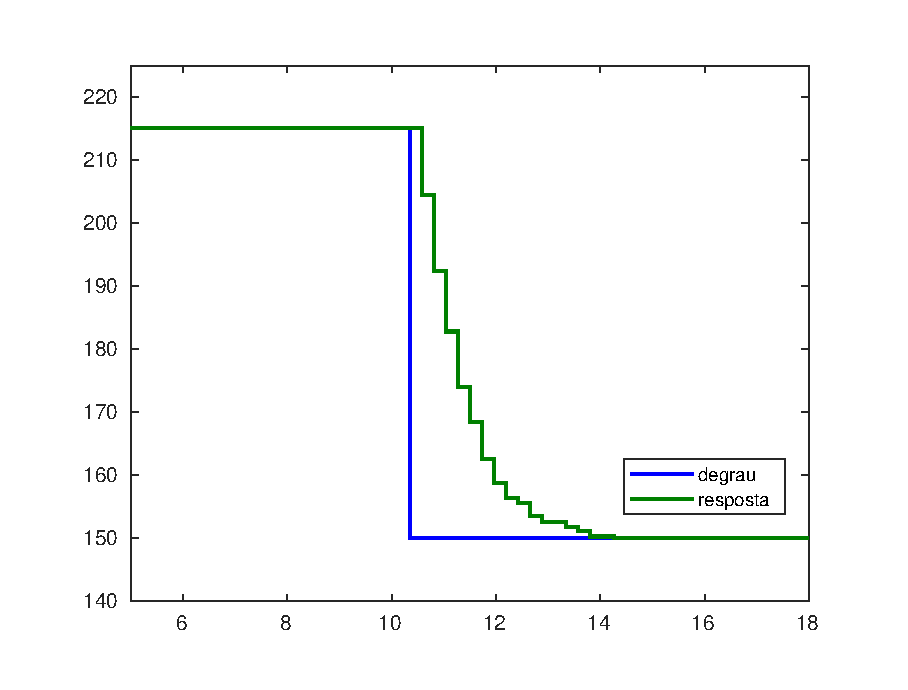
\includegraphics[width = 1\columnwidth]{Imagens/base_hilFase3}
    \fonte{Do autor}
    \label{fig:base_hilFase3}
  \end{subfigure}%
  \begin{subfigure}{.5\textwidth}
    \centering
    \caption{Ombro}
    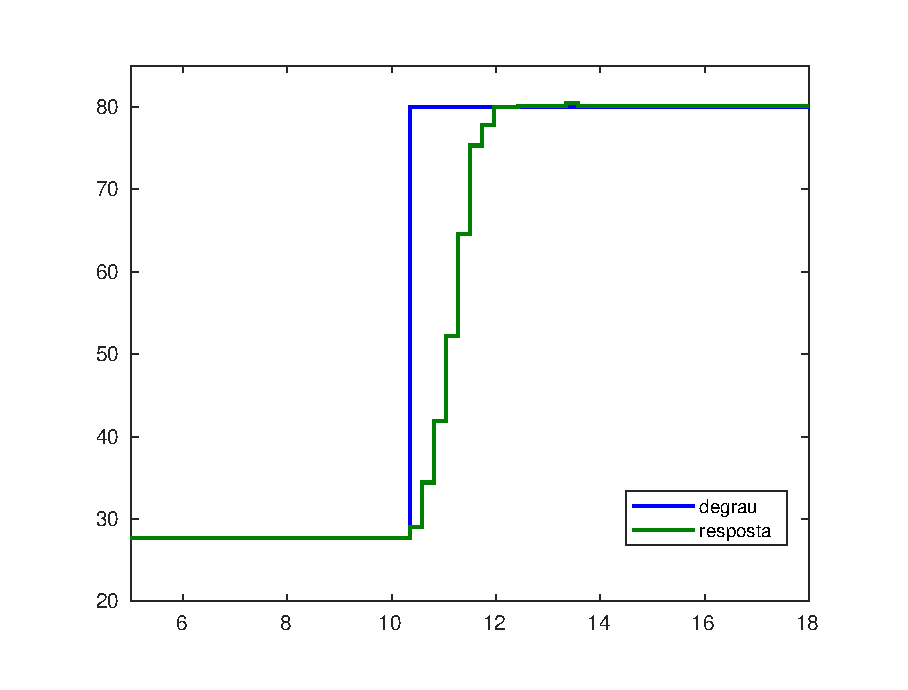
\includegraphics[width = 1\columnwidth]{Imagens/shoulder_hilFase3}
    \fonte{Do autor}
    \label{fig:shoulder_hilFase3}
  \end{subfigure}%
  \\
  \begin{subfigure}{\textwidth}
    \centering
    \caption{Cotovelo}
    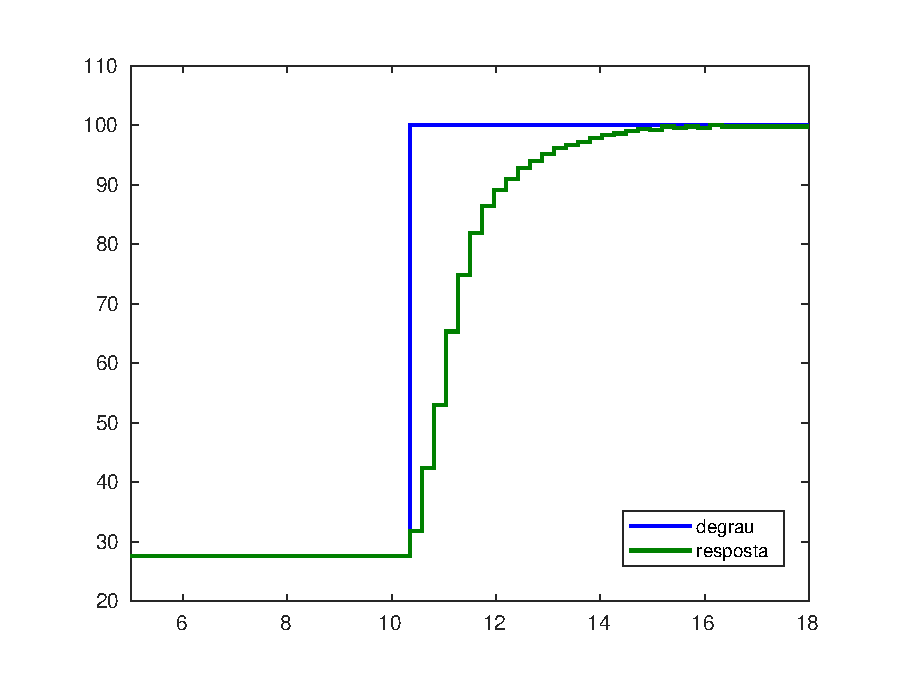
\includegraphics[width = 0.5\columnwidth]{Imagens/forearm_hilFase3}
    \fonte{Do autor}
    \label{fig:forearm_hilFase3}
  \end{subfigure}%
  
  \label{fig:hilFase3} 

\end{figure}

\section{Resumo do Capítulo}
\markright{\thesection ~~~ Resultados}

Este capítulo apresentou os resultados alcançados no projeto, apresentando a memória de cálculo,
explicitando como o sistema foi iplementado e expondo os resultados por meio dos gráficos. No próximo
capítulo são apresentadas as conclusões do projeto, como os resultados estão relacionados, são expostos, também, 
os problemas encontrados e são tecidas algumas sugestões para uma futura evolução do projeto.


\clearpage